\clearpage
\VerdierPhysicalPageAnchor{0087}%
\VerdierSemanticAnchor{ch1-3-2-2-dual-morphism}
Similarly, the morphism of $\operatorname{tr}_1(C)$:

\VerdierSemanticAnchor{ch1-3-2-2-eq3}
\begin{equation}
  \begin{tikzpicture}[>=stealth,baseline=(current bounding box.center)]
    \node (Z)  at (0,1.35) {$0$};
    \node (Y)  at (3.6,1.35) {$Y$};
    \node (X)  at (0,0) {$X$};
    \node (Yp) at (3.6,0) {$Y$};
    \draw[->] (Z) -- (Y);
    \draw[->] (Z) -- (X);
    \draw[->] (Y) -- node[right] {$\operatorname{id}_Y$} (Yp);
    \draw[->] (X) -- node[above] {$f$} (Yp);
  \end{tikzpicture}
  \tag{3.2.2.3}
\end{equation}

\VerdierSemanticAnchor{ch1-3-2-2-cone-entry-p}
yields, upon applying the cone functor, a morphism of
$\operatorname{comp}(C)$, functorial in $X\xrightarrow{f}Y$, (3.1.2.4):

\VerdierSemanticAnchor{ch1-3-2-2-eq4}
\begin{equation}
  p(f)\colon Y\longrightarrow c(f).
  \tag{3.2.2.4}
\end{equation}

\VerdierSemanticAnchor{ch1-3-2-2-comp-triangle}
We can therefore associate with every object $X\xrightarrow{f}Y$ of
$\operatorname{tr}_1(C)$ a triangle of $\operatorname{comp}(C)$:

\VerdierSemanticAnchor{ch1-3-2-2-eq5}
\begin{equation}
  X\xrightarrow{f}Y\xrightarrow{p(f)}c(f)\xrightarrow{q(f)}X[1].
  \tag{3.2.2.5}
\end{equation}

\VerdierSemanticAnchor{ch1-3-2-2-nonfunctoriality}
Notice that this triangle does not depend functorially on the object
$X\xrightarrow{f}Y$ of $\operatorname{tr}_1(C)$.
\VerdierSemanticAnchor{ch1-3-2-2-morphism-d-setup}
Indeed, let
$D=(g,h,a)\colon(X\xrightarrow{f}Y)\longrightarrow
(X'\xrightarrow{f'}Y')$
be a morphism of $\operatorname{tr}_1(C)$. We then obtain the diagram:

\VerdierSemanticAnchor{ch1-3-2-2-eq6}
\begin{equation}
  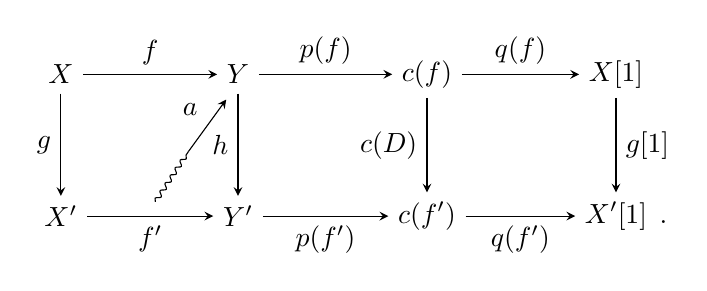
\begin{tikzpicture}[>=stealth,baseline=(current bounding box.center)]
    \node (X)   at (0,1.8) {$X$};
    \node (Y)   at (2.25,1.8) {$Y$};
    \node (C)   at (4.65,1.8) {$c(f)$};
    \node (Xs)  at (7.05,1.8) {$X[1]$};
    \node (Xp)  at (0,0) {$X'$};
    \node (Yp)  at (2.25,0) {$Y'$};
    \node (Cp)  at (4.65,0) {$c(f')$};
    \node (Xps) at (7.05,0) {$X'[1]$};
    \node[anchor=base west,inner sep=0pt,xshift=.08em] at (Xps.base east) {$.$};
    \draw[->] (X) -- node[above] {$f$} (Y);
    \draw[->] (Y) -- node[above] {$p(f)$} (C);
    \draw[->] (C) -- node[above] {$q(f)$} (Xs);
    \draw[->] (Xp) -- node[below] {$f'$} (Yp);
    \draw[->] (Yp) -- node[below] {$p(f')$} (Cp);
    \draw[->] (Cp) -- node[below] {$q(f')$} (Xps);
    \draw[->] (X) -- node[left] {$g$} (Xp);
    \draw[->] (Y) -- node[left] {$h$} (Yp);
    \draw[->] (C) -- node[left] {$c(D)$} (Cp);
    \draw[->] (Xs) -- node[right] {$g[1]$} (Xps);
    \draw[decorate,decoration={snake,amplitude=0.8pt,segment length=3.3pt}]
      (1.20,0.18) -- (1.62,0.82);
    \draw[->] (1.62,0.82) -- node[above left] {$a$} (2.10,1.48);
  \end{tikzpicture}
  \tag{3.2.2.6}
\end{equation}

\VerdierSemanticAnchor{ch1-3-2-2-square-commutativity}
Since the morphisms $p(f)$ and $q(f)$ are functorial in $f$, the last two
squares of this diagram are commutative, but the first square is commutative
only up to homotopy.
\VerdierSemanticAnchor{ch1-3-2-2-quotient-triangle}
Passing to the quotient by homotopies, we can associate with every object
$X\xrightarrow{f}Y$ of $\operatorname{Tr}_1(C)$ a triangle of $K(C)$:

\VerdierSemanticAnchor{ch1-3-2-2-eq7}
\begin{equation}
  X\xrightarrow{\dot f}Y\xrightarrow{\dot p(f)}c(f)
  \xrightarrow{\dot q(f)}X[1]
  \tag{3.2.2.7}
\end{equation}

\VerdierSemanticAnchor{ch1-3-2-2-homotopy-class-notation}
which depends functorially on $X\xrightarrow{f}Y$. (We denote by
$\dot f$, $\dot p(f)$, $\dot q(f)$ the classes modulo homotopy of the morphisms
$f$, $p(f)$, $q(f)$, respectively.)
\VerdierSemanticAnchor{ch1-3-2-2-triangle-functor}
We thus have a functor from the category $\operatorname{Tr}_1(C)$ to the
category of triangles of $K(C)$.
